\documentclass[11pt]{article}
\usepackage{graphicx}
\usepackage{booktabs}

\title{A Demo Manuscript}
\author{Demo Author}
\date{}

\begin{document}
\maketitle

\section{Introduction}
Figure~\ref{fig:res} summarises the main result, which is discussed below.
The text also contains an inline formula-like symbol: $x_1$ is written in math mode.

\section{Methods}
\begin{table}[h]
\centering
\begin{tabular}{lcr}
\toprule
setting & value & unit \\
temperature & 25 & C \\
pressure & 12 & MPa \\
\bottomrule
\end{tabular}
\end{table}

\section{Results}
The method is compared with earlier work \cite{sheng2021}.
Figure~\ref{fig:res} shows the comparison.

\begin{figure}[h]
\centering
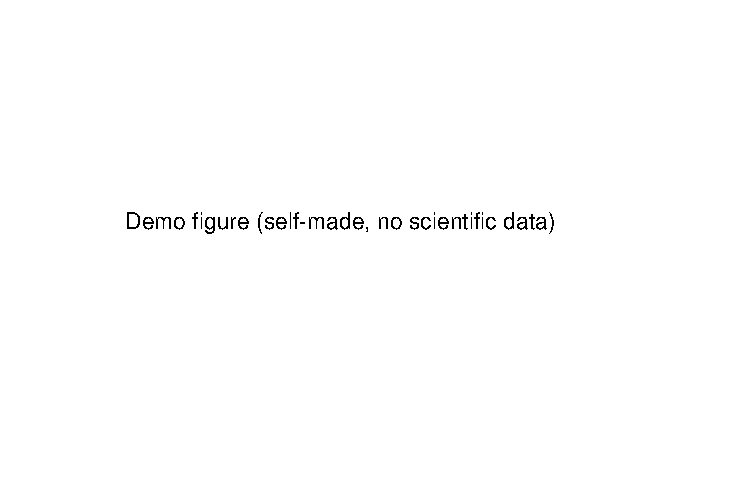
\includegraphics[width=0.8\linewidth]{figs/result.pdf}
\caption{Demo figure.}
\label{fig:res}
\end{figure}

\section{Conclusions}
The demo manuscript compiles and the template requirements are met.

\bibliographystyle{plain}
\bibliography{refs}

\end{document}
